\documentclass[11pt]{beamer}
\usetheme{CambridgeUS}
\usepackage[utf8]{inputenc}
\usepackage{amsmath}
\usepackage{amsfonts}
\usepackage{amssymb}
\usepackage{graphicx}
\usepackage{pgfpages}
\usepackage{framed}
\usepackage{xcolor}
\usepackage[most]{tcolorbox}
\usepackage{soul}
\usepackage{empheq}

\newcommand*{\itemimg}[1]{%
  \raisebox{-.3\baselineskip}{%
    \includegraphics[
      height=\baselineskip,
      width=\baselineskip,
      keepaspectratio,
    ]{#1}%
  }%
}

\newtcbox{\mymath}[1][]{%
    nobeforeafter, math upper, tcbox raise base,
    enhanced, colframe=blue!30!black,
    colback=blue!10, boxrule=1pt,
    #1}

\newcommand{\highlight}[1]{%
  \colorbox{yellow!100}{$\displaystyle#1$}}

\author{Giovanni Della Lunga\\{\footnotesize giovanni.dellalunga@unibo.it}}
%\title{1 - Introduction to Machine Learning}
%\title{2.1 - Data Pre-Processing}
\title{4.2 - Model Selection}
%\title{4.2 - Decision Trees}
%\title{6 - Text Vectorization}
%\title{7 - Classification for Text Analysis}
%\title{8 - Clustering for Text Similarity}
%\title{9 - Information Extraction}
\subtitle{} % (optional)
\setbeamercovered{transparent} 
%\institute{Introduction to Machine Learning for Finance} 
\date{Bologna - February-April, 2025} 

\begin{document}

\begin{frame}
\titlepage
\end{frame}

\AtBeginSection[]
{
%	\begin{frame}<beamer>
%  		\frametitle{Outline}
%  		\tableofcontents[currentsection]
%	\end{frame}
  	\begin{frame}
  		\vfill
  		\centering
  		\begin{beamercolorbox}	[sep=8pt,center,shadow=true,rounded=true]{title}  		\usebeamerfont{title}\insertsectionhead\par%
  		\end{beamercolorbox}
  		\vfill
  \end{frame}
}
\AtBeginSubsection{\frame{\subsectionpage}}


%	\begin{center}
%	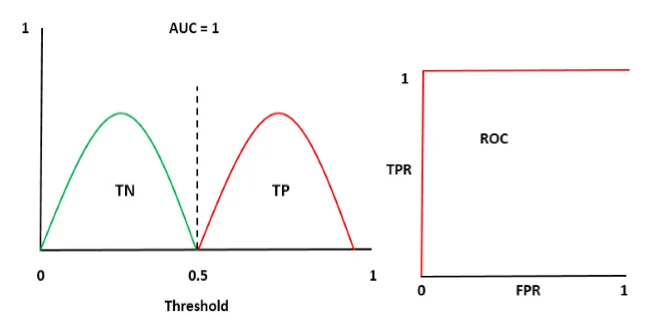
\includegraphics[scale=0.5]{../05-pictures/lesson-4-1_pic_4.png}
%	\end{center}
%..................................................................
%______________________________________________________________________________
%
%\section{Model Selection}

%\usepackage{booktabs}
%\usepackage{hyperref}


% Slide 1: Introduction
\begin{frame}{Introduction}
    \begin{itemize}
        \item Model selection is crucial for developing machine learning solutions.
        \item It involves choosing an algorithm and hyperparameters to optimize generalization.
        \item Balancing bias and variance is essential to prevent underfitting and overfitting.
        \item Cross-validation is a key technique for robust evaluation.
    \end{itemize}
\end{frame}

% Slide 2: Theoretical Foundations
\begin{frame}{Theoretical Foundations}
    \begin{itemize}
        \item Bias-variance tradeoff: high bias leads to underfitting, high variance leads to overfitting.
        \item K-fold cross-validation: partitions data into k subsets, ensuring fair validation.
        \item Each subset is used as validation once, while others are used for training.
    \end{itemize}
    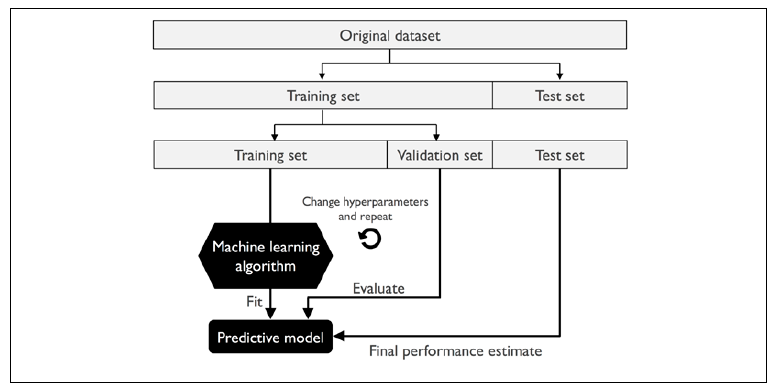
\includegraphics[width=0.8\textwidth]{../05-pictures/lesson-4-2_pic_0.png}
\end{frame}

% New Slide: Cross-Validation Explained
\begin{frame}{What is Cross-Validation?}
    \begin{itemize}
        \item Cross-validation is a resampling technique used to evaluate machine learning models.
        \item The dataset is split into multiple subsets (folds), and the model is trained and validated on different folds.
        \item The most common method is \textbf{K-fold cross-validation}, where:
        \begin{itemize}
            \item The dataset is divided into K equally-sized subsets.
            \item The model is trained on K-1 subsets and tested on the remaining subset.
            \item This process repeats K times, with each subset used as the test set once.
        \end{itemize}
        \item The final model performance is computed as the average of the results across all folds.
    \end{itemize}
    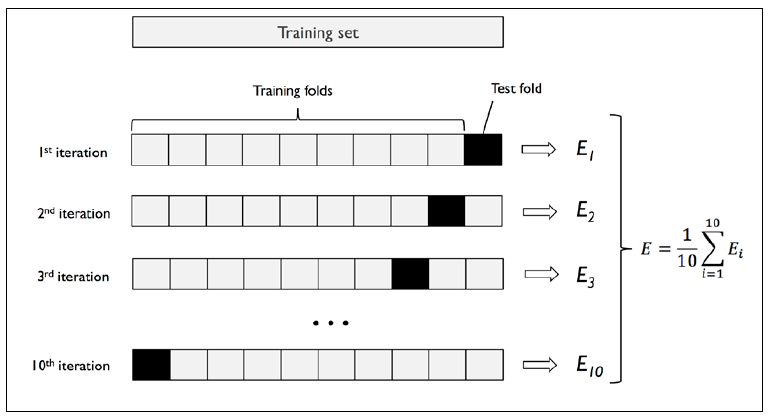
\includegraphics[width=0.8\textwidth]{../05-pictures/lesson-4-2_pic_1.png}
\end{frame}

% Slide 3: Practical Model Selection
\begin{frame}{Practical Model Selection Using Python}
    \begin{itemize}
        \item Compare multiple models using cross-validation.
        \item Example: Predicting housing prices using Scikit-learn.
        \item \texttt{cross\_val\_score} function evaluates model performance using folds.
    \end{itemize}
    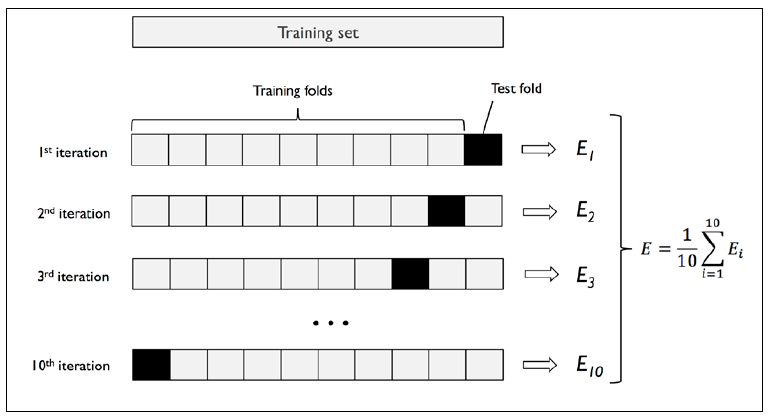
\includegraphics[width=0.8\textwidth]{../05-pictures/lesson-4-2_pic_1.png}
\end{frame}

% Slide 4: Python Code Example
\begin{frame}[fragile]{Python Code Example}
    \begin{itemize}
        \item Import necessary libraries and load dataset.
        \item Split data into training and testing sets.
        \item Define multiple models (Linear Regression, Random Forest, etc.).
        \item Perform 5-fold cross-validation and compute $R^2$ scores.
    \end{itemize}
    \begin{verbatim}
    from sklearn.model_selection import cross_val_score
    models = {
        "Linear Regression": LinearRegression(),
        "Random Forest": RandomForestRegressor(n_estimators=100, random_state=42)
    }
    results = {}
    for name, model in models.items():
        scores = cross_val_score(model, X_train, y_train, cv=5, scoring='r2')
        results[name] = np.mean(scores)
    \end{verbatim}
\end{frame}

% Slide 5: Interpretation of Results
\begin{frame}{Interpretation of Results}
    \begin{itemize}
        \item Compare R$^2$ scores to determine the best model.
        \item Consider interpretability, computational efficiency, and robustness.
        \item Example: Linear Regression vs. Random Forest.
    \end{itemize}
\end{frame}

% Slide 6: Hyperparameter Tuning
\begin{frame}[fragile]{Hyperparameter Tuning}
    \begin{itemize}
        \item Optimizing hyperparameters improves model performance.
        \item Common techniques: Grid Search, Random Search.
        \item Example: Tuning Random Forest with GridSearchCV.
    \end{itemize}
    \begin{verbatim}
    param_grid = {
        'n_estimators': [50, 100, 200],
        'max_depth': [None, 10, 20]
    }
    grid_search = GridSearchCV(RandomForestRegressor(), param_grid, cv=5, scoring='r2')
    grid_search.fit(X_train, y_train)
    \end{verbatim}
\end{frame}

% Slide 7: Pipelines
\begin{frame}{Pipelines}
    \begin{itemize}
        \item Ensures consistency across training and testing.
        \item Chains preprocessing steps with model training.
        \item Simplifies hyperparameter tuning.
    \end{itemize}
    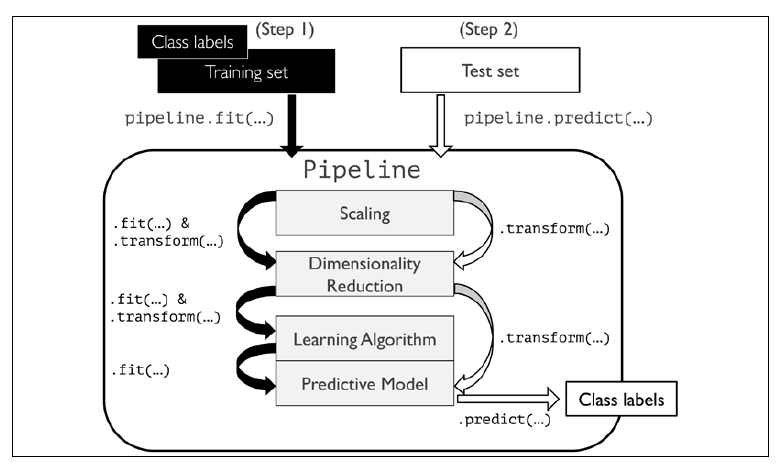
\includegraphics[width=0.8\textwidth]{../05-pictures/lesson-4-2_pic_2.png}
\end{frame}

% Slide 8: Learning Curves
\begin{frame}{Learning Curves}
    \begin{itemize}
        \item Show model performance evolution with training data size.
        \item Help diagnose underfitting and overfitting.
        \item Training and validation error curves provide key insights.
    \end{itemize}
\end{frame}

% Slide 9: Learning Curves in Python
\begin{frame}{Learning Curves in Python}
    \begin{itemize}
        \item Example: Linear Regression vs. Decision Tree learning curves.
        \item Use Scikit-learn's \texttt{learning\_curve} function.
    \end{itemize}
    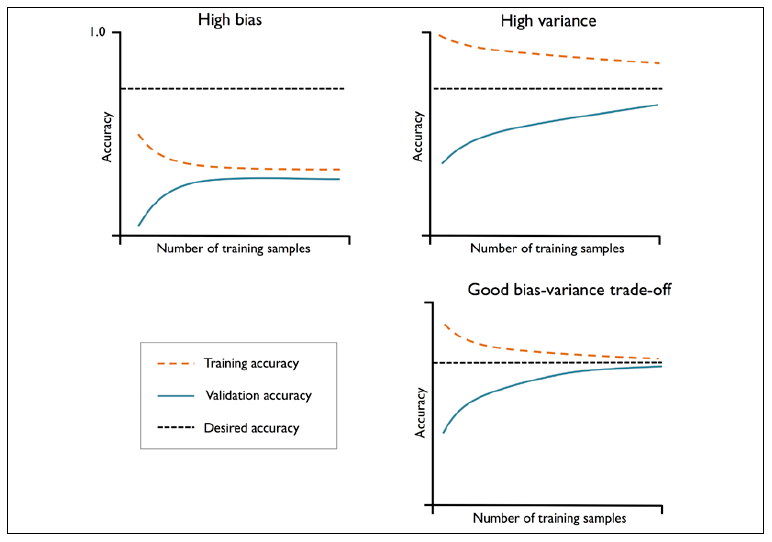
\includegraphics[width=0.8\textwidth]{../05-pictures/lesson-4-2_pic_3.png}
\end{frame}

% Slide 10: Grid Search
\begin{frame}{Grid Search}
    \begin{itemize}
        \item Systematically evaluates hyperparameter combinations.
        \item Example: Random Forest tuning.
        \item Trade-off between computational cost and performance.
    \end{itemize}
\end{frame}

% Slide 11: Conclusion
\begin{frame}{Conclusion}
    \begin{itemize}
        \item Model selection and hyperparameter tuning are crucial.
        \item Cross-validation ensures robust evaluation.
        \item Use learning curves to optimize models effectively.
    \end{itemize}
\end{frame}

% Slide 12: References
\begin{frame}{References}
    \begin{itemize}
        \item Python Machine Learning, Third Edition by Sebastian Raschka.
        \item Code Repository: \url{https://github.com/rasbt/python-machine-learning-book-3rd-edition}
    \end{itemize}
\end{frame}

\end{document}

%______________________________________________________________________________
%
\section{References and Credits}
%===================================================================================================
\begin{frame}{Bibliography}
\begin{thebibliography}{9}

\setbeamertemplate{bibliography item}[book]

\bibitem{1} John C. Hull, \textit{Machine Learning in Business: An Introduction to the World of Data Science}, Amazon, 2019.

\bibitem{2} Paul Wilmott, \textit{Machine Learning: An Applied Mathematics Introduction}, Panda Ohana Publishing, 2019.

\end{thebibliography}
\end{frame}
%===================================================================================================
\end{document}

%..................................................................
\begin{frame}{Notebook Reference}
\begin{columns}[T] % align columns
\begin{column}{.48\textwidth}
        \begin{itemize}
		\item \textbf{chapter-1-4} Notebook 
		\item[] In this notebook you will find an example of applying the metrics discussed in this section applied to a simple case of credit risk. Knowledge of logistic regression and credit risk issues is assumed.
        \end{itemize}
\end{column}%
\hfill%
\begin{column}{.48\textwidth}
    %\fbox{
        \includegraphics[width=\linewidth]{../05-pictures/letscode.png}
    %}
\end{column}%
\end{columns}
\end{frame}
%..................................................................
\begin{frame}{}
\begin{itemize}
\item 
\end{itemize}
\end{frame}
%..................................................................
\begin{frame}{}
\begin{itemize}
\item 
\end{itemize}
\end{frame}
%..................................................................
\begin{frame}{}
\begin{itemize}
\item 
\end{itemize}
\end{frame}
%..................................................................
\begin{frame}{}
\begin{itemize}
\item 
\end{itemize}
\end{frame}
